\section{Tip speed analysis}

One of the differences between the different tip speeds was the data density. For faster speed less data was taken, while slower speeds had more data taken. This was due to the rate in which the AFM takes in data - the AFM was set to take in the maximum rate of data throughout the whole process. This was done to maximise the volume of data usable for the binning process (as seen in chapter 5). 

For 0.1 and 0.5Hz, the data rate was more than enough the support the processing of the curves, while 2Hz had significantly less data, and required a more involved fitting, with generally a lower bitsize setting used in the script - increasing the noise in the averaged curve.

For 0.1 and 0.5Hz, the data rate was more than enough the support the processing of the curves, while 2Hz had significantly less data, and required a more involved fitting, with generally a lower bitsize setting used in the script - increasing the noise in the averaged curve.

% 0.6mM Section
\subsection*{0.6mM}
\begin{figure}[h!]
\centering
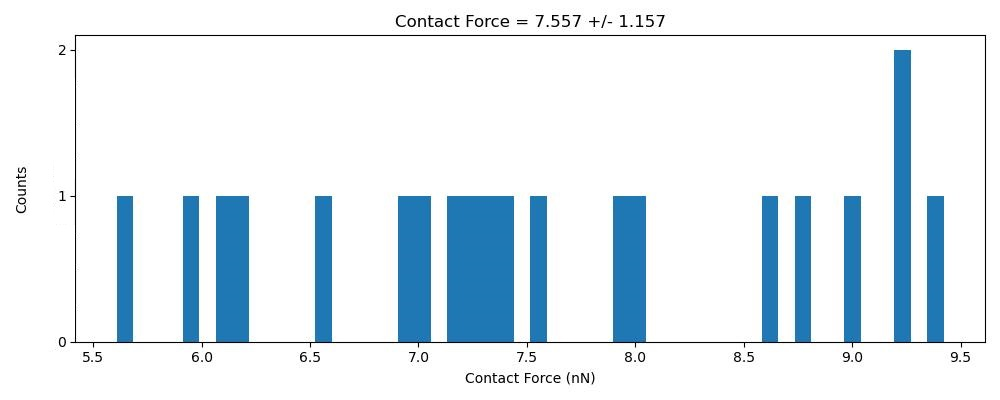
\includegraphics[width=\textwidth]{chapter7/Tip speed/0.6mM/approach_f_c_hist.jpg}
\caption{Approach force-current histogram at 0.6mM}
\end{figure}

\begin{figure}[h!]
\centering
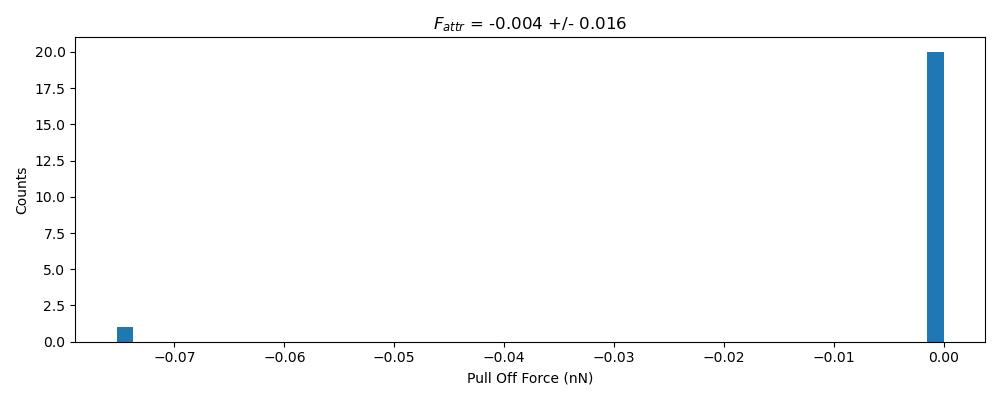
\includegraphics[width=\textwidth]{chapter7/Tip speed/0.6mM/retract_f_a_hist.jpg}
\caption{Retract force-amplitude histogram at 0.6mM}
\end{figure}

% 1.6mM Section
\subsection*{1.6mM}
\subsubsection*{Site 1 2Hz}
\begin{figure}[h!]
\centering
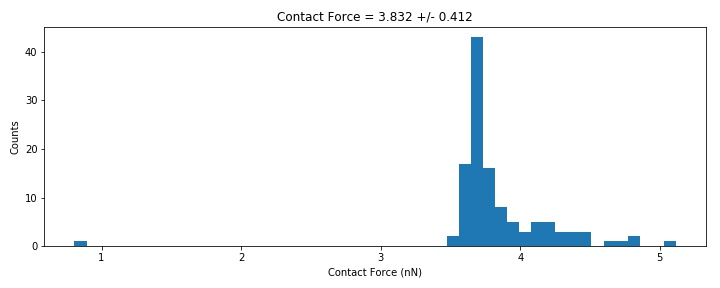
\includegraphics[width=\textwidth]{chapter7/Tip speed/1.6mM/S1_2Hz/approach_f_c_hist.jpg}
\caption{Site 1 Approach force-current histogram at 2Hz and 1.6mM}
\end{figure}

\begin{figure}[h!]
\centering
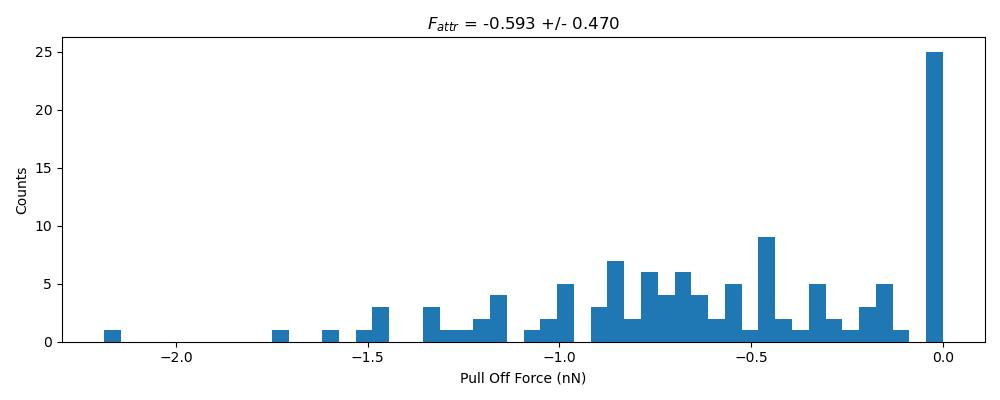
\includegraphics[width=\textwidth]{chapter7/Tip speed/1.6mM/S1_2Hz/retract_f_a_hist.jpg}
\caption{Site 1 Retract force-amplitude histogram at 2Hz and 1.6mM}
\end{figure}


\section{JPK Forcemapping}

One of the limitations of using the interpertaion software is that it assumes that all curves are of the same shape. This is not the case for a range of sites.

Due to the differences between the AFMs, and potentially the way the AFMs were used to measure the interactions, the "shelf" seen was more of a snap to contact point in the curve. This meant that the shelf seen in the previous AFM, may have been the point in which the tip snapped to the surface, and the older AFM may not have been able to detect or measure this sudden change in the way the new one has. 

Due to the limited window in which this AFM was available, it was not possible to explore this interaction further, but it is promising that this shelf feature is present across multiple AFMs and sites.